% move all configuration stuff into one file so we can focus on the content
\documentclass[aspectratio=169,hyperref={pdfpagelabels=false,colorlinks=true,linkcolor=white,urlcolor=blue},t]{beamer}

%%%%%%%%%%%%%%%%%%%%%%%%%%%%%%%%%%%%%%%%%%%%%%%%%%%%%%%%%%%%%%%%%%%%%%%%%%%%%%%%%%
%%%%%%%%%%%%%%%%%%%%%%%%%%%%%%%%%%%%%%%%%%%%%%%%%%%%%%%%%%%%%%%%%%%%%%%%%%%%%%%%%%
% packages
\usepackage{pict2e}
\usepackage{epic}
\usepackage{amsmath,amsfonts,amssymb}
\usepackage{units}
\usepackage{fancybox}
\usepackage[absolute,overlay]{textpos} 
\usepackage{media9} % avi2flv: "C:\Program Files\ffmpeg\bin\ffmpeg.exe" -i TuneFreqFilterbank.avi -b 600k -s 441x324 -r 15 -acodec copy TuneFreqFilterbank.flv
\usepackage{animate}
\usepackage{gensymb}
\usepackage{multirow}
\usepackage{silence}
\usepackage[backend=bibtex,style=ieee]{biblatex}
\AtEveryCitekey{\iffootnote{\tiny}{}}
\addbibresource{references}

%%%%%%%%%%%%%%%%%%%%%%%%%%%%%%%%%%%%%%%%%%%%%%%%%%%%%%%%%%%%%%%%%%%%%%%%%%%%%%%%%%
%%%%%%%%%%%%%%%%%%%%%%%%%%%%%%%%%%%%%%%%%%%%%%%%%%%%%%%%%%%%%%%%%%%%%%%%%%%%%%%%%%
% relative paths
\graphicspath{{graph/}}


%%%%%%%%%%%%%%%%%%%%%%%%%%%%%%%%%%%%%%%%%%%%%%%%%%%%%%%%%%%%%%%%%%%%%%%%%%%%%%%%%%
%%%%%%%%%%%%%%%%%%%%%%%%%%%%%%%%%%%%%%%%%%%%%%%%%%%%%%%%%%%%%%%%%%%%%%%%%%%%%%%%%%
% units
\setlength{\unitlength}{1mm}

%%%%%%%%%%%%%%%%%%%%%%%%%%%%%%%%%%%%%%%%%%%%%%%%%%%%%%%%%%%%%%%%%%%%%%%%%%%%%%%%%%
%%%%%%%%%%%%%%%%%%%%%%%%%%%%%%%%%%%%%%%%%%%%%%%%%%%%%%%%%%%%%%%%%%%%%%%%%%%%%%%%%%
% theme & layout
\usetheme{Frankfurt}
\beamertemplatenavigationsymbolsempty
%\setbeamertemplate{frametitle}[smoothbars theme]
\setbeamertemplate{frametitle}
{
    \begin{beamercolorbox}[ht=1.8em,wd=\paperwidth]{frametitle}
        \vspace{-.1em}%
        \hspace{.2em}{\strut\insertframetitle\strut}
        
        \hspace{.2em}\small\strut\insertframesubtitle\strut
        %\hfill
        %
\includegraphics[height=.8cm,keepaspectratio]{CenterMusicTechnology-solid-2lines-white-CoAtag}
        
    \end{beamercolorbox}
    \begin{textblock*}{100mm}(11.6cm,.7cm)
        \includegraphics[height=.8cm,keepaspectratio]{logo_GTCMT_black}
    \end{textblock*}
}

% set this to ensure bulletpoints without subsections
\usepackage{remreset}
\makeatletter
\@removefromreset{subsection}{section}
\makeatother
\setcounter{subsection}{1}

%---------------------------------------------------------------------------------
% appearance
\setbeamercolor{structure}{fg=gtgold}
\setbeamercovered{transparent} %invisible
\setbeamercolor{bibliography entry author}{fg=black}
\setbeamercolor*{bibliography entry title}{fg=black}
\setbeamercolor*{bibliography entry note}{fg=black}

%\usepackage{pgfpages}
%\setbeameroption{show notes}
%\setbeameroption{show notes on second screen=right}
%---------------------------------------------------------------------------------
% fontsize
\let\Tiny=\tiny

%%%%%%%%%%%%%%%%%%%%%%%%%%%%%%%%%%%%%%%%%%%%%%%%%%%%%%%%%%%%%%%%%%%%%%%%%%%%%%%%%%
%%%%%%%%%%%%%%%%%%%%%%%%%%%%%%%%%%%%%%%%%%%%%%%%%%%%%%%%%%%%%%%%%%%%%%%%%%%%%%%%%%
% warnings
\pdfsuppresswarningpagegroup=1
\WarningFilter{biblatex}{Patching footnotes failed}
\WarningFilter{latexfont}{Font shape}
\WarningFilter{latexfont}{Some font shapes}
\WarningFilter{gensymb}{Not defining}



\subtitle{Part 6.1: Tonal Analysis Introduction}

%%%%%%%%%%%%%%%%%%%%%%%%%%%%%%%%%%%%%%%%%%%%%%%%%%%%%%%%%%%%%%%%%%%%%%%%%%%%
\begin{document}
    % generate title page
	

\begin{frame}
    \titlepage
    %\vspace{-5mm}
    \begin{flushright}
        \href{http://www.gtcmt.gatech.edu}{\includegraphics[height=.8cm,keepaspectratio]{logo_GTCMT_black}}
    \end{flushright}
\end{frame}


    \section[overview]{lecture overview}
        \begin{frame}{tonal analysis}{overview}
            \begin{itemize}
                \item   \textbf{text book}  
                    \begin{itemize}
                        \item   \href{http://ieeexplore.ieee.org/xpl/articleDetails.jsp?tp=&arnumber=&}{\underline{\textit{Chapter 5: Tonal Analysis} (pp.~85--98)}}
                    \end{itemize}
                \bigskip
                \item<2->   \textbf{lecture content}
                    \begin{itemize}
                        \item<2->   human pitch perception
                        \item<3->   pitch notation in music
                        \item<4->   tonal concepts: intervals, chords, key, etc.\ in music
                    \end{itemize}
            \end{itemize}
        \end{frame}

    \section[intro]{introduction}
        \begin{frame}{tonal analysis}{introduction}
            \begin{itemize}
                \item pitch is one of the most important parameters describing musical characteristics
                    \begin{itemize}
                        \item   modal
                        \item   harmonic
                        \item   melodic
                        \item   intonation
                    \end{itemize}
                \item<2-> related ACA tasks
                    \begin{itemize}
                        \item   key detection
                        \item   harmony \& chord detection
                        \item   fundamental frequency detection
                        \item   tuning frequency \& temperament estimation
                    \end{itemize}
            \end{itemize}
        \end{frame}

    \section[perception]{pitch perception}
         \begin{frame}{pitch}{pitch perception 1/2}
            \begin{block}{\textbf{definition (American Standards Association)}}
                pitch is that attribute of auditory sensation in terms of which sounds may be ordered on a musical scale\footfullcite{asa_acoustical_1960}
            \end{block}
            \bigskip    
            \begin{itemize}
                \item<2->   temporal variations in pitch give rise to a sense of melody
                \item<2->   closely related to frequency, but \textbf{subjective}

                \bigskip
                \item<3->[$\Rightarrow$]   assigning a pitch value to a sound means \textbf{specifying the frequency of a pure tone having the same subjective pitch} as the sound
            \end{itemize}
        \end{frame}
        
        \begin{frame}{pitch}{pitch perception 2/2}
            \vspace{-2mm}
            \begin{itemize}
                \item	dominant \textit{fundamental} frequency ($f_0,2f_0,3f_0,\ldots$)
                    \vspace{-3mm}
                    \figwithmatlab{Harmonics}

                
                \item<2->	higher frequency $\Rightarrow$ higher pitch (mono-dimensional)

                \item<3->	\textbf{non-linear}:
                    \begin{itemize}
                        \item	perceptual pitch distance $\neq$ frequency distance
                        
                        \item<4->	models for psycho-acoustic/physiological data
                            \begin{itemize}
                                \item	\textit{Mel} scale (equal pitch distance)

                                \item<5->	\textit{Bark} scale (critical band width)

                                \item<6->	frequency location (basilar membrane)
                            \end{itemize}
                    \end{itemize}
            \end{itemize}
        \end{frame}
        \begin{frame}{pitch}{pitch perception --- non-linearity}
            \figwithmatlab{PerceptualPitch}
            \only<2-3>{
            \begin{eqnarray*}
                \text{\textbf{Fant}:} &          \mathfrak{m}_\mathrm{F}(f) = 1000\cdot \log_{2}\left(1 + \frac{f}{\unit[1000]{Hz}} \right)\\
                \text{\textbf{O'Shaughnessy}:} & \mathfrak{m}_\mathrm{S}(f) = 2595\cdot \log_{10}\left(1 + \frac{f}{\unit[700]{Hz}} \right)\\
                \pause
                &                       \mathfrak{m}_\mathrm{S}(f) = 1127\cdot \log\left(1 + \frac{f}{\unit[700]{Hz}} \right)
            \end{eqnarray*}
            }
            \only<4>{
            \begin{eqnarray*}
                \text{\textbf{Schr\"oder}:} &         \mathfrak{z}_\mathrm{S}(f) = 7\cdot\arcsinh\left( \frac{f}{\unit[650]{Hz}} \right) \\
                \text{\textbf{Terhardt}:} &         \mathfrak{z}_\mathrm{T}(f) = 13.3\cdot\arctan\left( 0.75\cdot\frac{f}{\unit[1000]{Hz}} \right) \\
                \text{\textbf{Zwicker}:} &          \mathfrak{z}_Z(f) = 13\cdot\atan\left( 0.76\cdot\frac{f}{\unit[1000]{Hz}} \right) + 3.5\cdot \atan\left( \frac{f}{\unit[7500]{Hz}} \right) 
            \end{eqnarray*}
            }
            \only<5>{
                \begin{eqnarray*}
                    \text{\textbf{ERB}:} &         \mathfrak{e}(f) = 9.26 \log \left( 1 + \frac{f}{228.7} \right)  \\
                    \text{\textbf{Cochlear Map}:} &          \mathfrak{x}(f)	= \frac{1}{2.1} \log_{10}\left( \frac{f}{165.4} + 1 \right)  
                \end{eqnarray*}
            }
        \end{frame}

        \begin{frame}{pitch}{pitch perception --- dimensions}
            \textbf{2 dimensions of musical pitch}
            \begin{itemize}
                \item   \textbf{tone height}: monotonic relationship to frequency (increasing frequency $\Rightarrow$ increasing pitch)
                \item<2->   \textbf{tone chroma}: two tones separated by octave sound similar (same \textit{pitch class})
                \only<2>{\vspace{-10mm}\figwithmatlab{PitchHelix}}
            \end{itemize}
        \end{frame}

    \section[musical]{pitch in music}
        \begin{frame}{pitch}{musical pitch --- pitch classes 1/2}
            each octave is split into $12$ pitch classes
            \begin{figure}
            \scalebox{.8}
            {
                \begin{footnotesize}
\begin{picture}(70,40)
	\setcounter{iXOffset}{0}
	\setcounter{iYOffset}{5}
	\setcounter{iXBlockSize}{10}
	\setcounter{iYBlockSize}{35}

	% white keys
	\put(\value{iXOffset}, \value{iYOffset})
		{\framebox(\value{iXBlockSize}, \value{iYBlockSize})[b] {\footnotesize{\shortstack[c]{$C$\\ \ }}}}

	\addtocounter{iXOffset}{\value{iXBlockSize}}
	\put(\value{iXOffset}, \value{iYOffset})
		{\framebox(\value{iXBlockSize}, \value{iYBlockSize})[b] {\footnotesize{\shortstack[c]{$D$\\ \ }}}}

	\addtocounter{iXOffset}{\value{iXBlockSize}}
	\put(\value{iXOffset}, \value{iYOffset})
		{\framebox(\value{iXBlockSize}, \value{iYBlockSize})[b] {\footnotesize{\shortstack[c]{$E$\\ \ }}}}

	\addtocounter{iXOffset}{\value{iXBlockSize}}
	\put(\value{iXOffset}, \value{iYOffset})
		{\framebox(\value{iXBlockSize}, \value{iYBlockSize})[b] {\footnotesize{\shortstack[c]{$F$\\ \ }}}}

	\addtocounter{iXOffset}{\value{iXBlockSize}}
	\put(\value{iXOffset}, \value{iYOffset})
		{\framebox(\value{iXBlockSize}, \value{iYBlockSize})[b] {\footnotesize{\shortstack[c]{$G$\\ \ }}}}

	\addtocounter{iXOffset}{\value{iXBlockSize}}
	\put(\value{iXOffset}, \value{iYOffset})
		{\framebox(\value{iXBlockSize}, \value{iYBlockSize})[b] {\footnotesize{\shortstack[c]{$A$\\ \ }}}}
	\addtocounter{iXOffset}{\value{iXBlockSize}}
	
	\put(\value{iXOffset}, \value{iYOffset})
		{\framebox(\value{iXBlockSize}, \value{iYBlockSize})[b] {\footnotesize{\shortstack[c]{$B$\\ \ }}}}

	\setcounter{iDistance}{\value{iXBlockSize}}
	\setcounter{iXOffset}{7}
	\setcounter{iYOffset}{16}
	\setcounter{iXBlockSize}{3}
	\setcounter{iYBlockSize}{23}
	
	\put(\value{iXOffset}, \value{iYOffset})
		{\colorbox{black}{ \framebox(\value{iXBlockSize}, \value{iYBlockSize})[b] {\footnotesize{\shortstack[c]{\textcolor {white}{$C\sharp$}\\ \textcolor {white}{$D\flat$}\\ \ }}}}}

	\addtocounter{iXOffset}{\value{iDistance}}
	
	\put(\value{iXOffset}, \value{iYOffset})
		{\colorbox{black}{ \framebox(\value{iXBlockSize}, \value{iYBlockSize})[b] {\footnotesize{\shortstack[c]{\textcolor {white}{$D\sharp$}\\ \textcolor {white}{$E\flat$}\\ \ }}}}}

	\addtocounter{iXOffset}{\value{iDistance}}
	\addtocounter{iXOffset}{\value{iDistance}}
	
	\put(\value{iXOffset}, \value{iYOffset})
		{\colorbox{black}{ \framebox(\value{iXBlockSize}, \value{iYBlockSize})[b] {\footnotesize{\shortstack[c]{\textcolor {white}{$F\sharp$}\\ \textcolor {white}{$G\flat$}\\ \ }}}}}

	\addtocounter{iXOffset}{\value{iDistance}}
	
	\put(\value{iXOffset}, \value{iYOffset})
		{\colorbox{black}{ \framebox(\value{iXBlockSize}, \value{iYBlockSize})[b] {\footnotesize{\shortstack[c]{\textcolor {white}{$G\sharp$}\\ \textcolor {white}{$A\flat$}\\ \ }}}}}

	\addtocounter{iXOffset}{\value{iDistance}}
	
	\put(\value{iXOffset}, \value{iYOffset})
		{\colorbox{black}{ \framebox(\value{iXBlockSize}, \value{iYBlockSize})[b] {\footnotesize{\shortstack[c]{\textcolor {white}{$A\sharp$}\\ \textcolor {white}{$B\flat$}\\ \ }}}}}

\end{picture}
\end{footnotesize}

            }
            \end{figure}

            \vspace{-8mm}
            \begin{footnotesize}
                \begin{table}
                    \centering
                    \begin{tabular}{cccccccccccc} %{\textwidth}{@{\extracolsep{\fill}}ccccccccccccc}
                        \\ \hline
                        \bf{\emph{Index}}	 & \bf{\emph{Name}}	 & \bf{\emph{Solfège Name}}	 & \bf{\emph{$\Delta\mathrm{ST}$}}\\ 
                         \hline
                        \bf{$0$}	 & $C$	 & Do	 & 1\\
                        \bf{$2$}	 & $D$	 & Re	 & 2\\
                        \bf{$4$}	 & $E$	 & Mi	 & 2\\
                        \bf{$5$}	 & $F$	 & Fa	 & 1\\
                        \bf{$7$}	 & $G$	 & Sol	 & 2\\
                        \bf{$9$}	 & $A$	 & La	 & 2\\
                        \bf{$11$}	 & $B$	 & Si	 & 2\\
                    \end{tabular}
                \end{table}
            \end{footnotesize}
        \end{frame}
        
        \begin{frame}{pitch}{musical pitch --- pitch classes 2/2}
            \begin{footnotesize}
                \begin{table}
                    \centering
                    \begin{tabular}{cccccccccccc} %{\textwidth}{@{\extracolsep{\fill}}ccccccccccccc}
                        \\ \hline
                        \bf{\emph{$0$}}	 & \bf{\emph{$1$}}	 & \bf{\emph{$2$}}	 & \bf{\emph{$3$}}	 & \bf{\emph{$4$}}	 & \bf{\emph{$5$}}	 & \bf{\emph{$6$}}	 & \bf{\emph{$7$}}	 & \bf{\emph{$8$}}	 & \bf{\emph{$9$}}	 & \bf{\emph{$10$}}	 & \bf{\emph{$11$}}\\ 
                         \hline
                        \bf{$C$}	 & $C\sharp / D\flat$	 & $D$	 & $D\sharp / E\flat$	 & E	 & $F$	 & $F\sharp / G\flat$	 & $G$	 & $G\sharp / A\flat$	 & $A$	 & $A\sharp / B\flat$	 & $B$\\
                    \end{tabular}
                \end{table}
            \end{footnotesize}

            \only<2>{
            \begin{figure}
                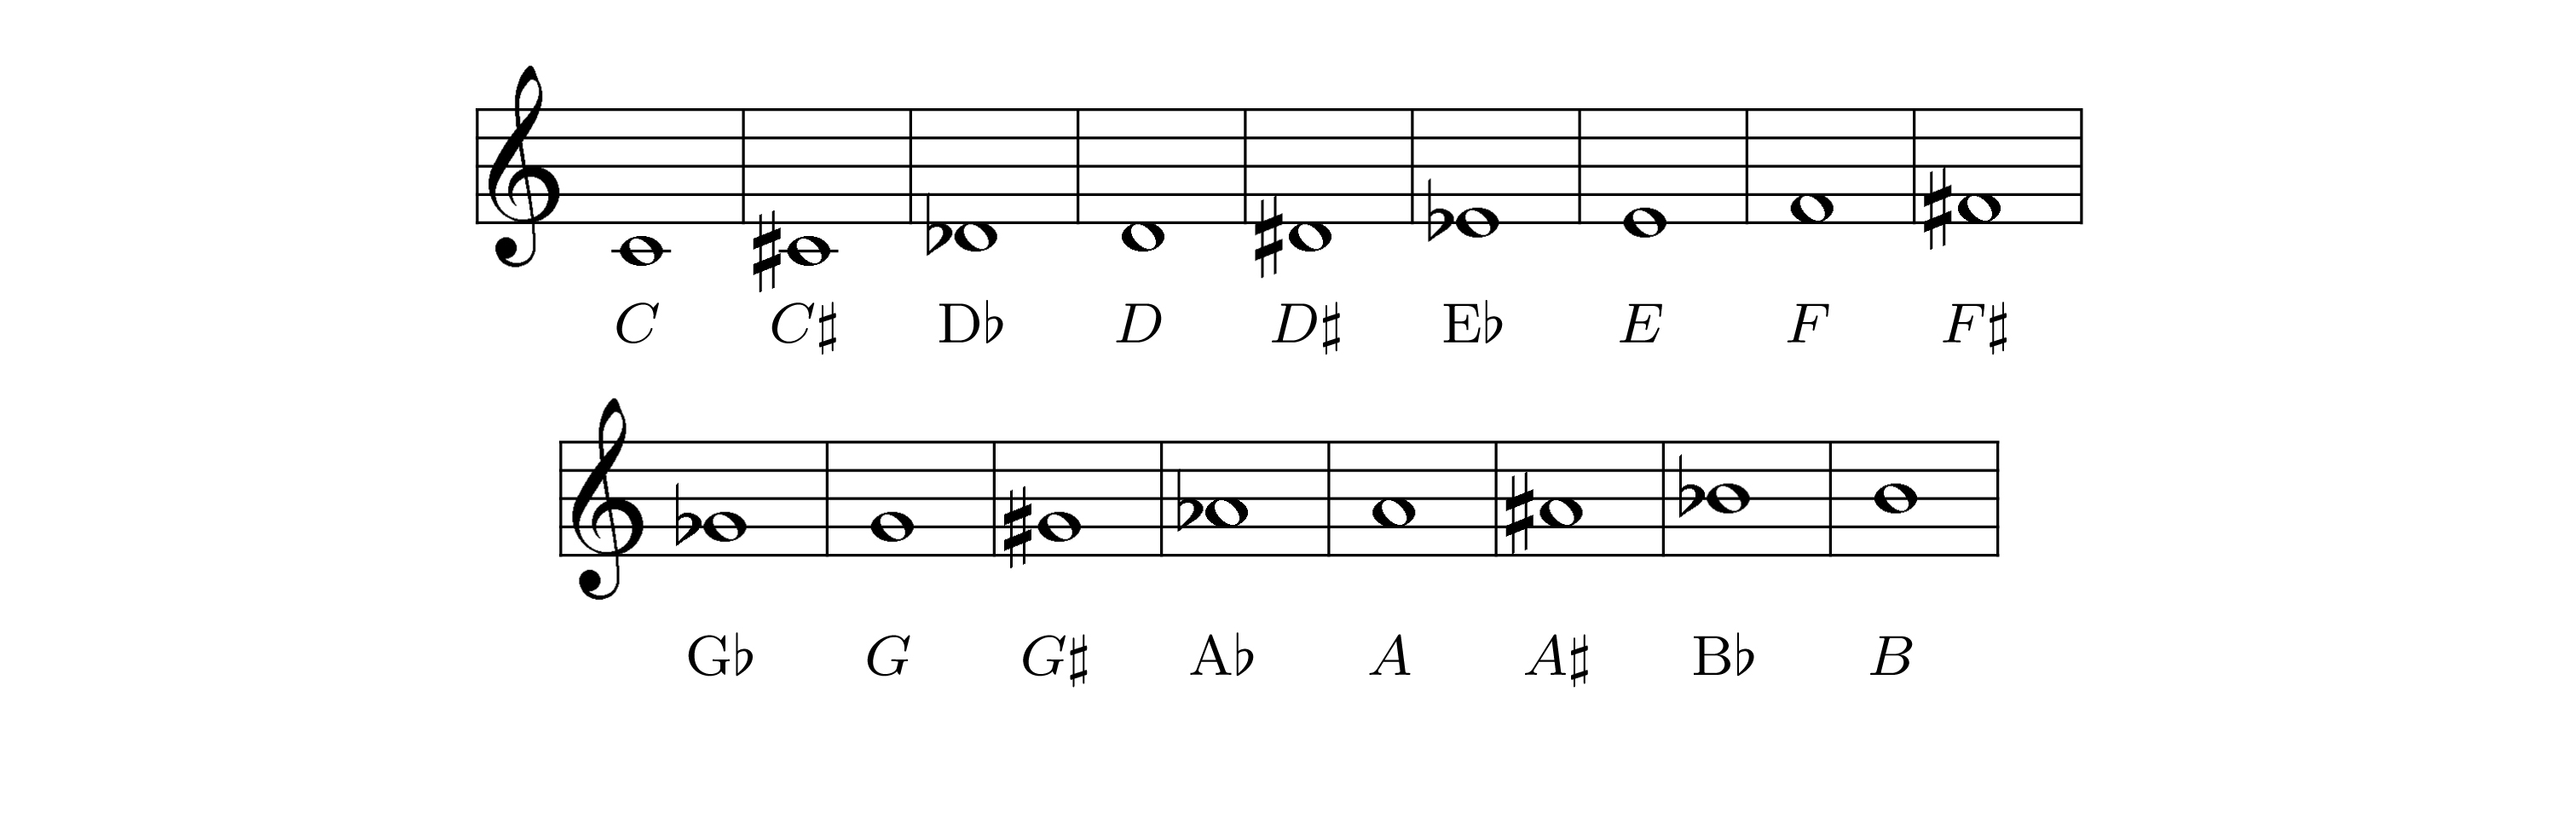
\includegraphics{pitch_pitches}
            \end{figure}}
        \end{frame}
        
        \begin{frame}{pitch}{musical pitch --- intervals}
            \vspace{-4mm}
            \begin{figure}
                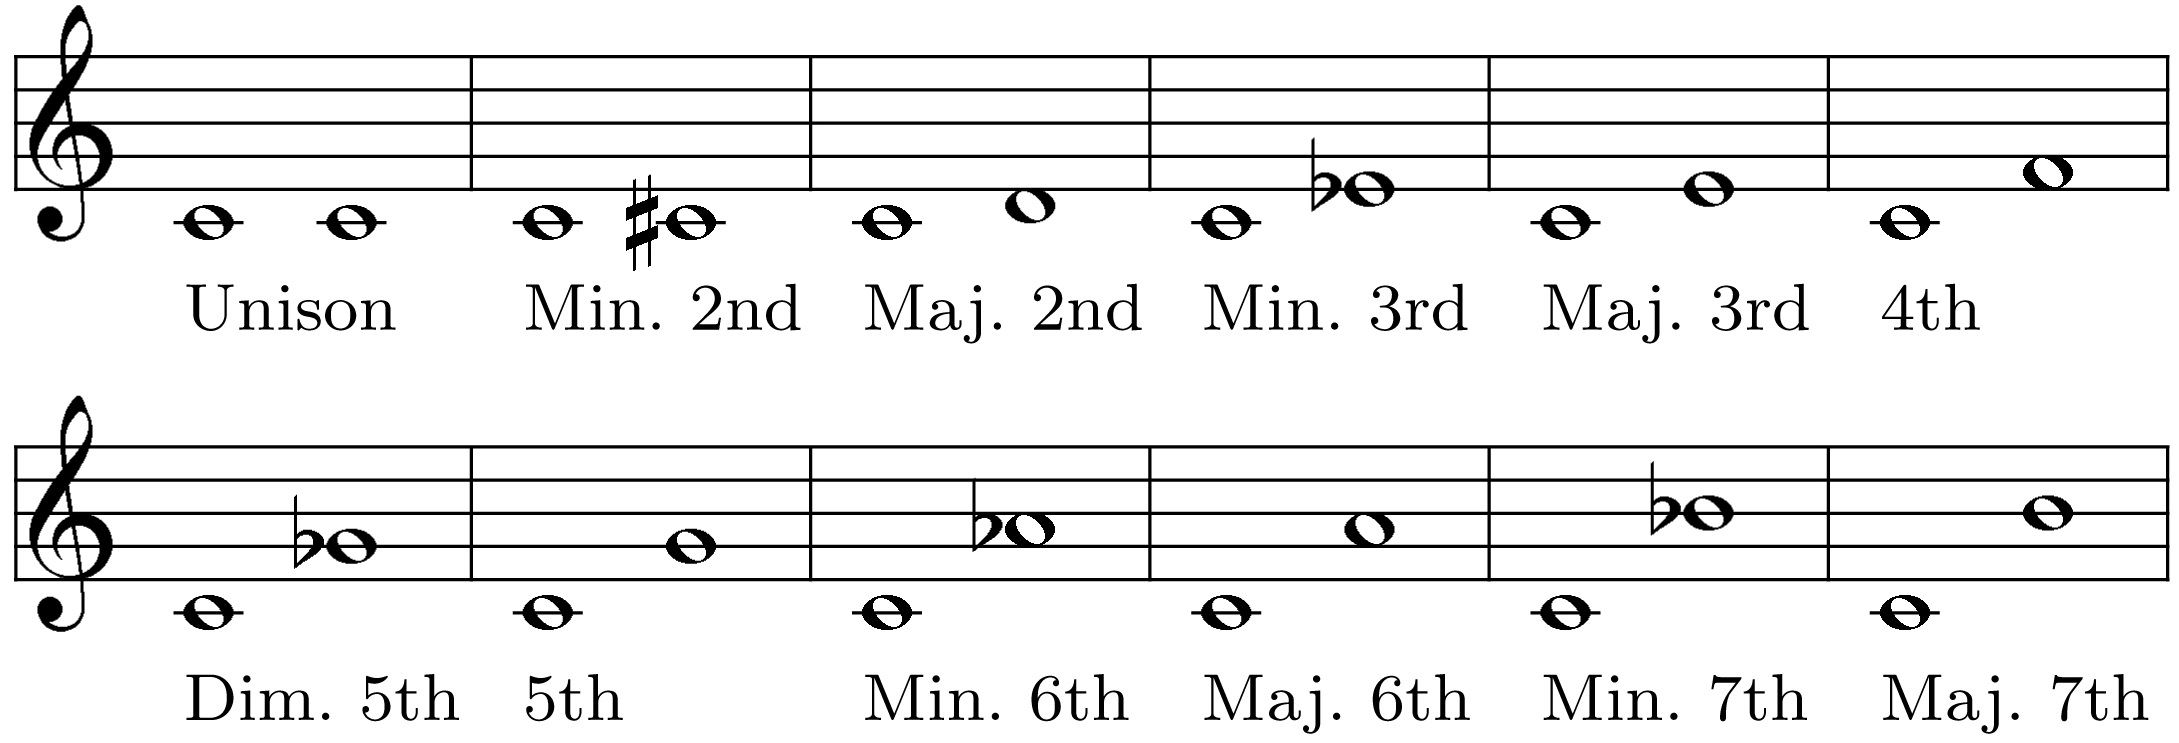
\includegraphics[scale=.7]{pitch_intervals}
            \end{figure}

            \pause
            \vspace{-6mm}
            \begin{scriptsize}
                \begin{table}
                    \centering
                    \begin{tabular}{lccccccccccc} %{\textwidth}{@{\extracolsep{\fill}}ccccccccccccc}
                        \\ \hline
                        \bf{\emph{Interval}}	 & \bf{\emph{Enharmonic Equivalent}}	 & \bf{\emph{$\Delta\mathrm{ST}$}}\\ 
                         \hline
                        \bf{Unison}	 & Diminished Second	 & 0\\
                        \bf{Minor Second}	 & Augmented Unison	 & 1\\
                        \bf{(Major) Second}	 & Diminished Third	 & 2\\
                        \bf{Minor Third}	 & Augmented Second	 & 3\\
                        \bf{Major Third}	 & Diminished Fourth	 & 4\\
                        \bf{(Perfect) Fourth}	 & Augmented Third	 & 5\\
                        \bf{Augmented Fourth}	 & Diminished Fifth/Tritone	 & 6\\
                        \bf{(Perfect) Fifth}	 & Diminished Sixth	 & 7\\
                        \bf{Minor Sixth}	 & Augmented Fifth	 & 8\\
                        \bf{Major Sixth}	 & Diminished Seventh	 & 9\\
                        \bf{Minor Seventh}	 & Augmented Sixth	 & 10\\
                        \bf{Major Seventh}	 & Diminished Octave	 & 11\\
                        \bf{(Perfect) Octave}	 & Augmented Seventh	 & 12\\
                    \end{tabular}
                \end{table}
            \end{scriptsize}
        \end{frame}
        
        \begin{frame}{pitch}{musical pitch --- tonic \& mode}
            \begin{itemize}
                \item	\textbf{tonic}: first scale degree
                        \pause
                        \begin{itemize}
                            \item	most ``important'' pitch class
                        \end{itemize}
                
                \item<2->	\textbf{mode}: set of pitch relationships (seconds)
                        \pause
                        \begin{itemize}
                            \item	Major: 2, 2, 1, 2, 2, 2, 1
                            \item	Minor: 2, 1, 2, 2, 1, 2, 2
                        \end{itemize}
                \only<2->{\begin{figure}[t]
                    \centering
                    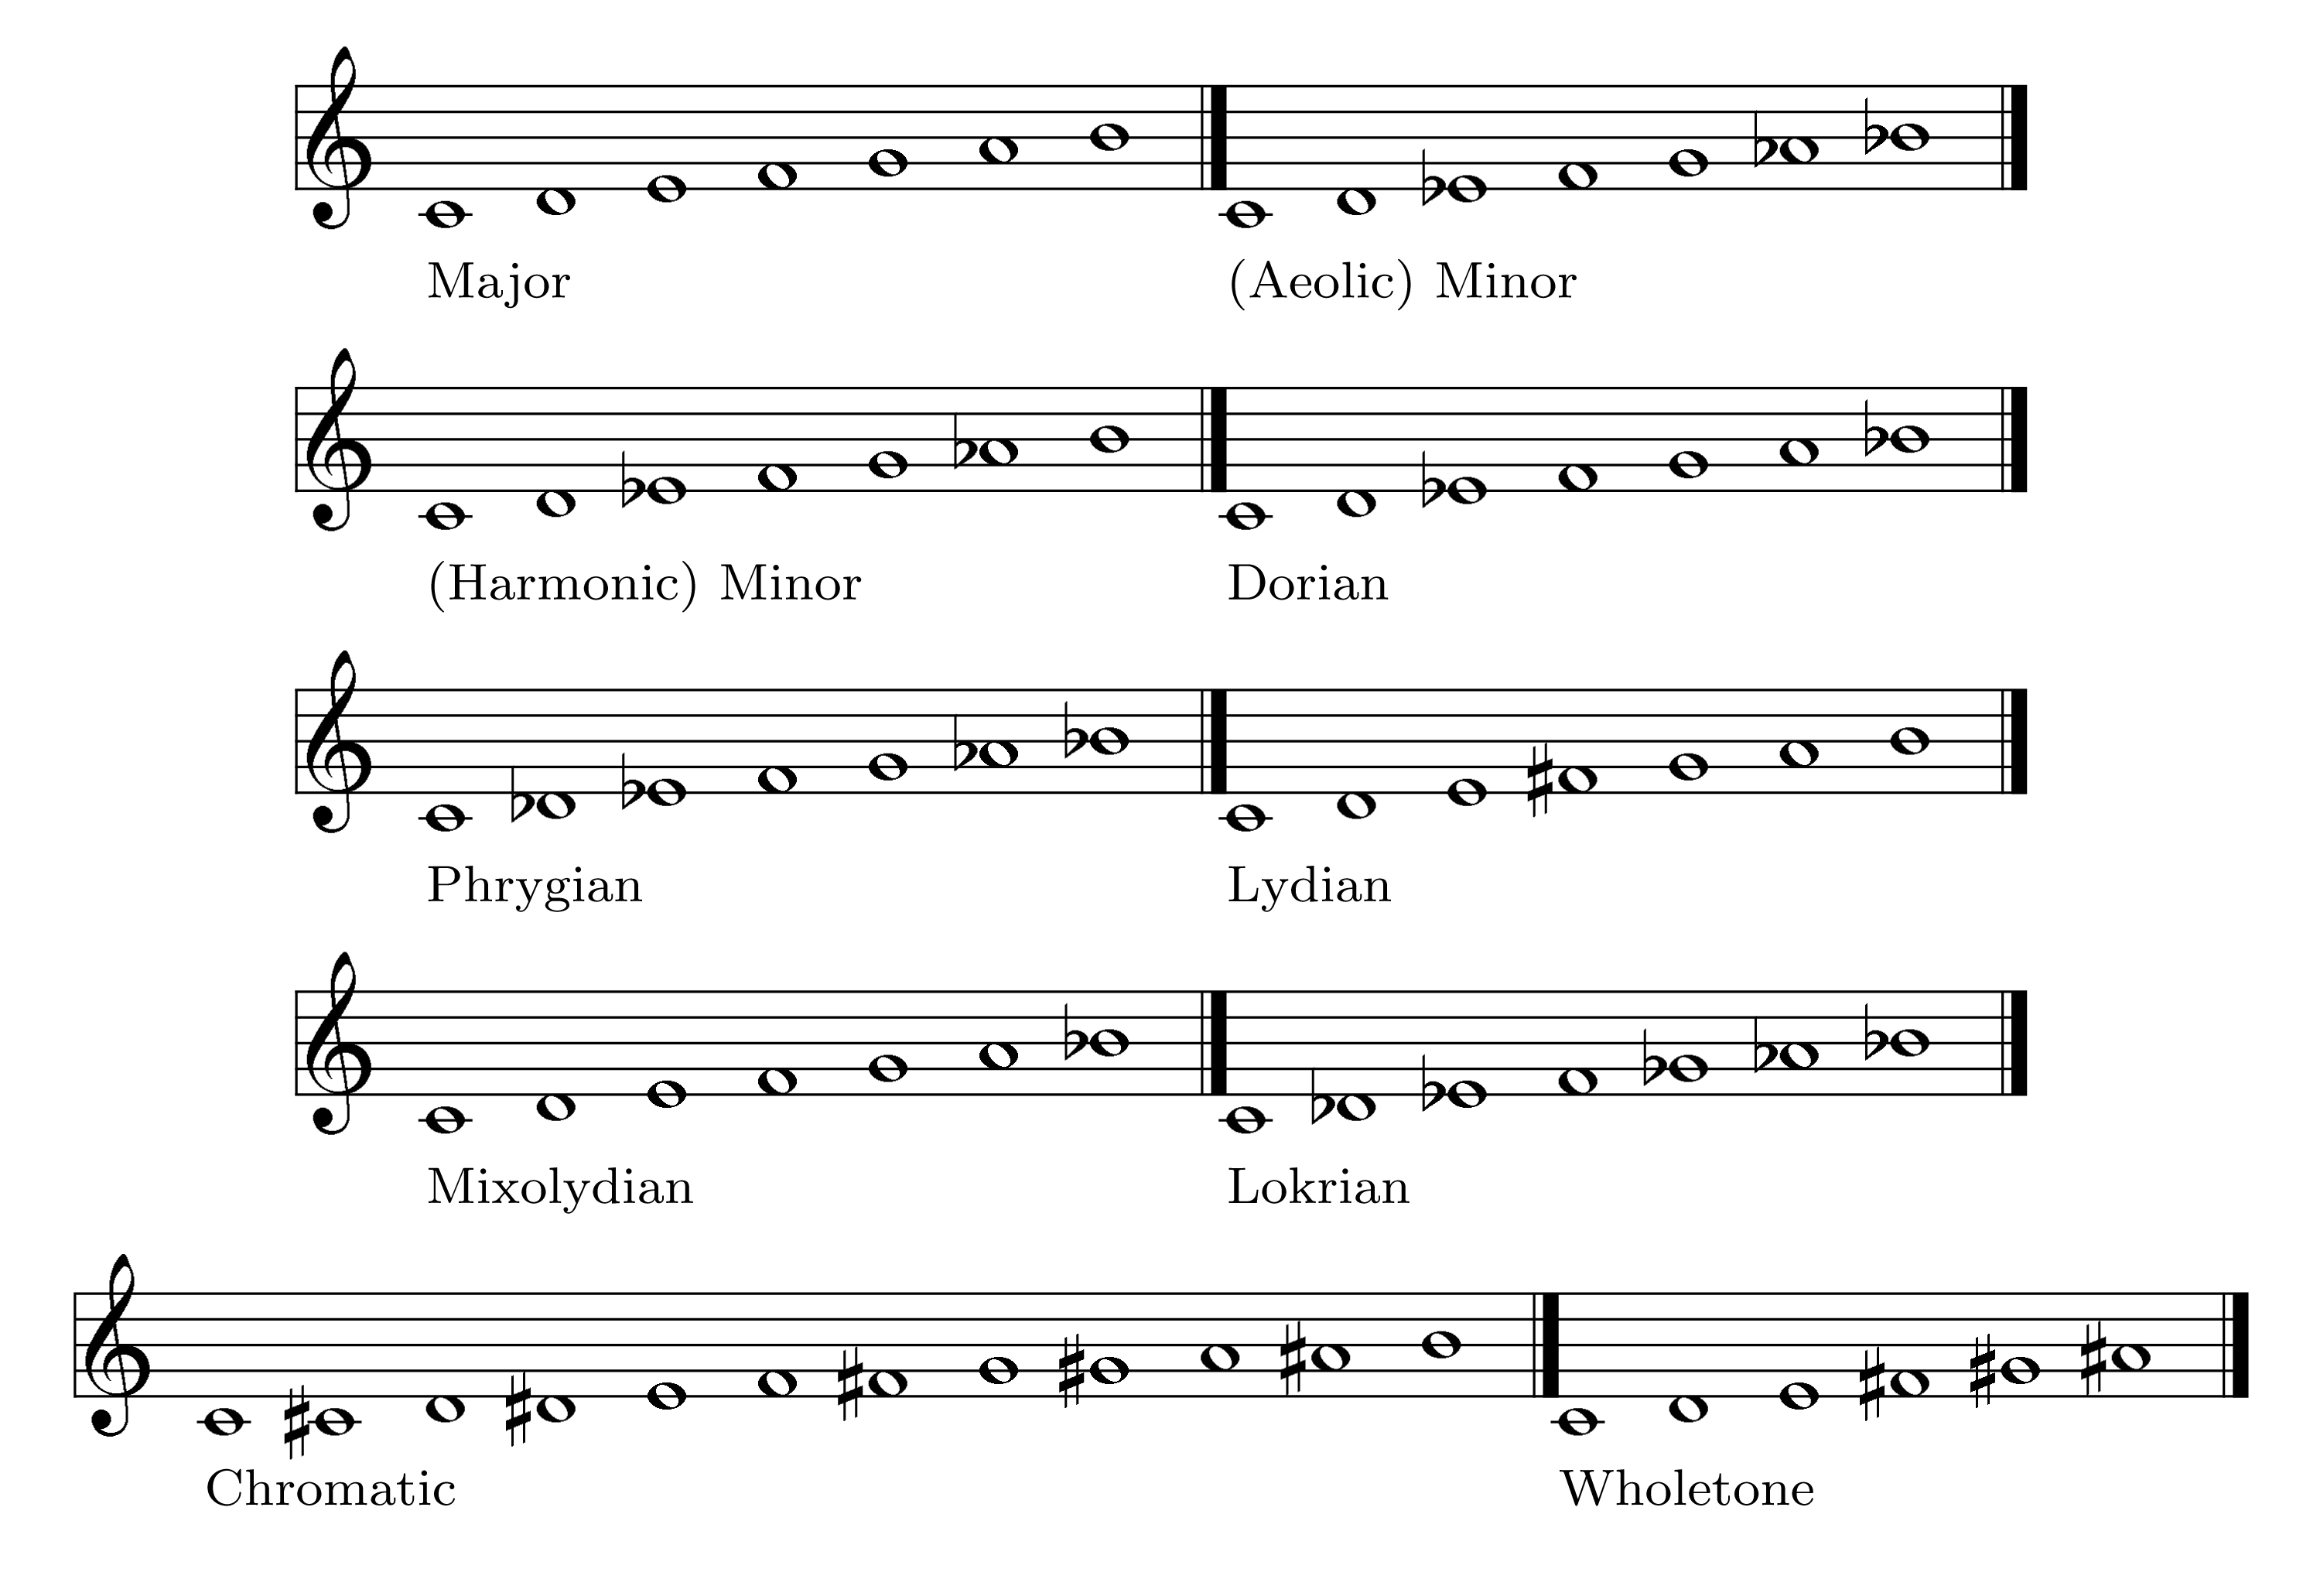
\includegraphics[scale=.6]{pitch_modes}
                \end{figure}
                }
            \end{itemize}
        \end{frame}
        
        \begin{frame}{pitch}{musical pitch --- key \& key signature 1/2}
            \begin{itemize}
                \item	\textbf{key}:\\ defined by \textit{tonic} (root note) and \textit{mode}
                        
                        \begin{itemize}
                            \item<2->	defines a set of pitch classes constructing both  pitch and harmonic content
                            
                            \item<3->	modulations (local key changes): common in various styles, uncommon in others
                        \end{itemize}
                \item<4->	\textbf{key signature}:\\ indicates current key with accidentals (score notation)
            \end{itemize}
        \end{frame}
        
        \begin{frame}{pitch}{musical pitch --- key \& key signature 2/2}
                \begin{figure}[t]
                    \centering
                    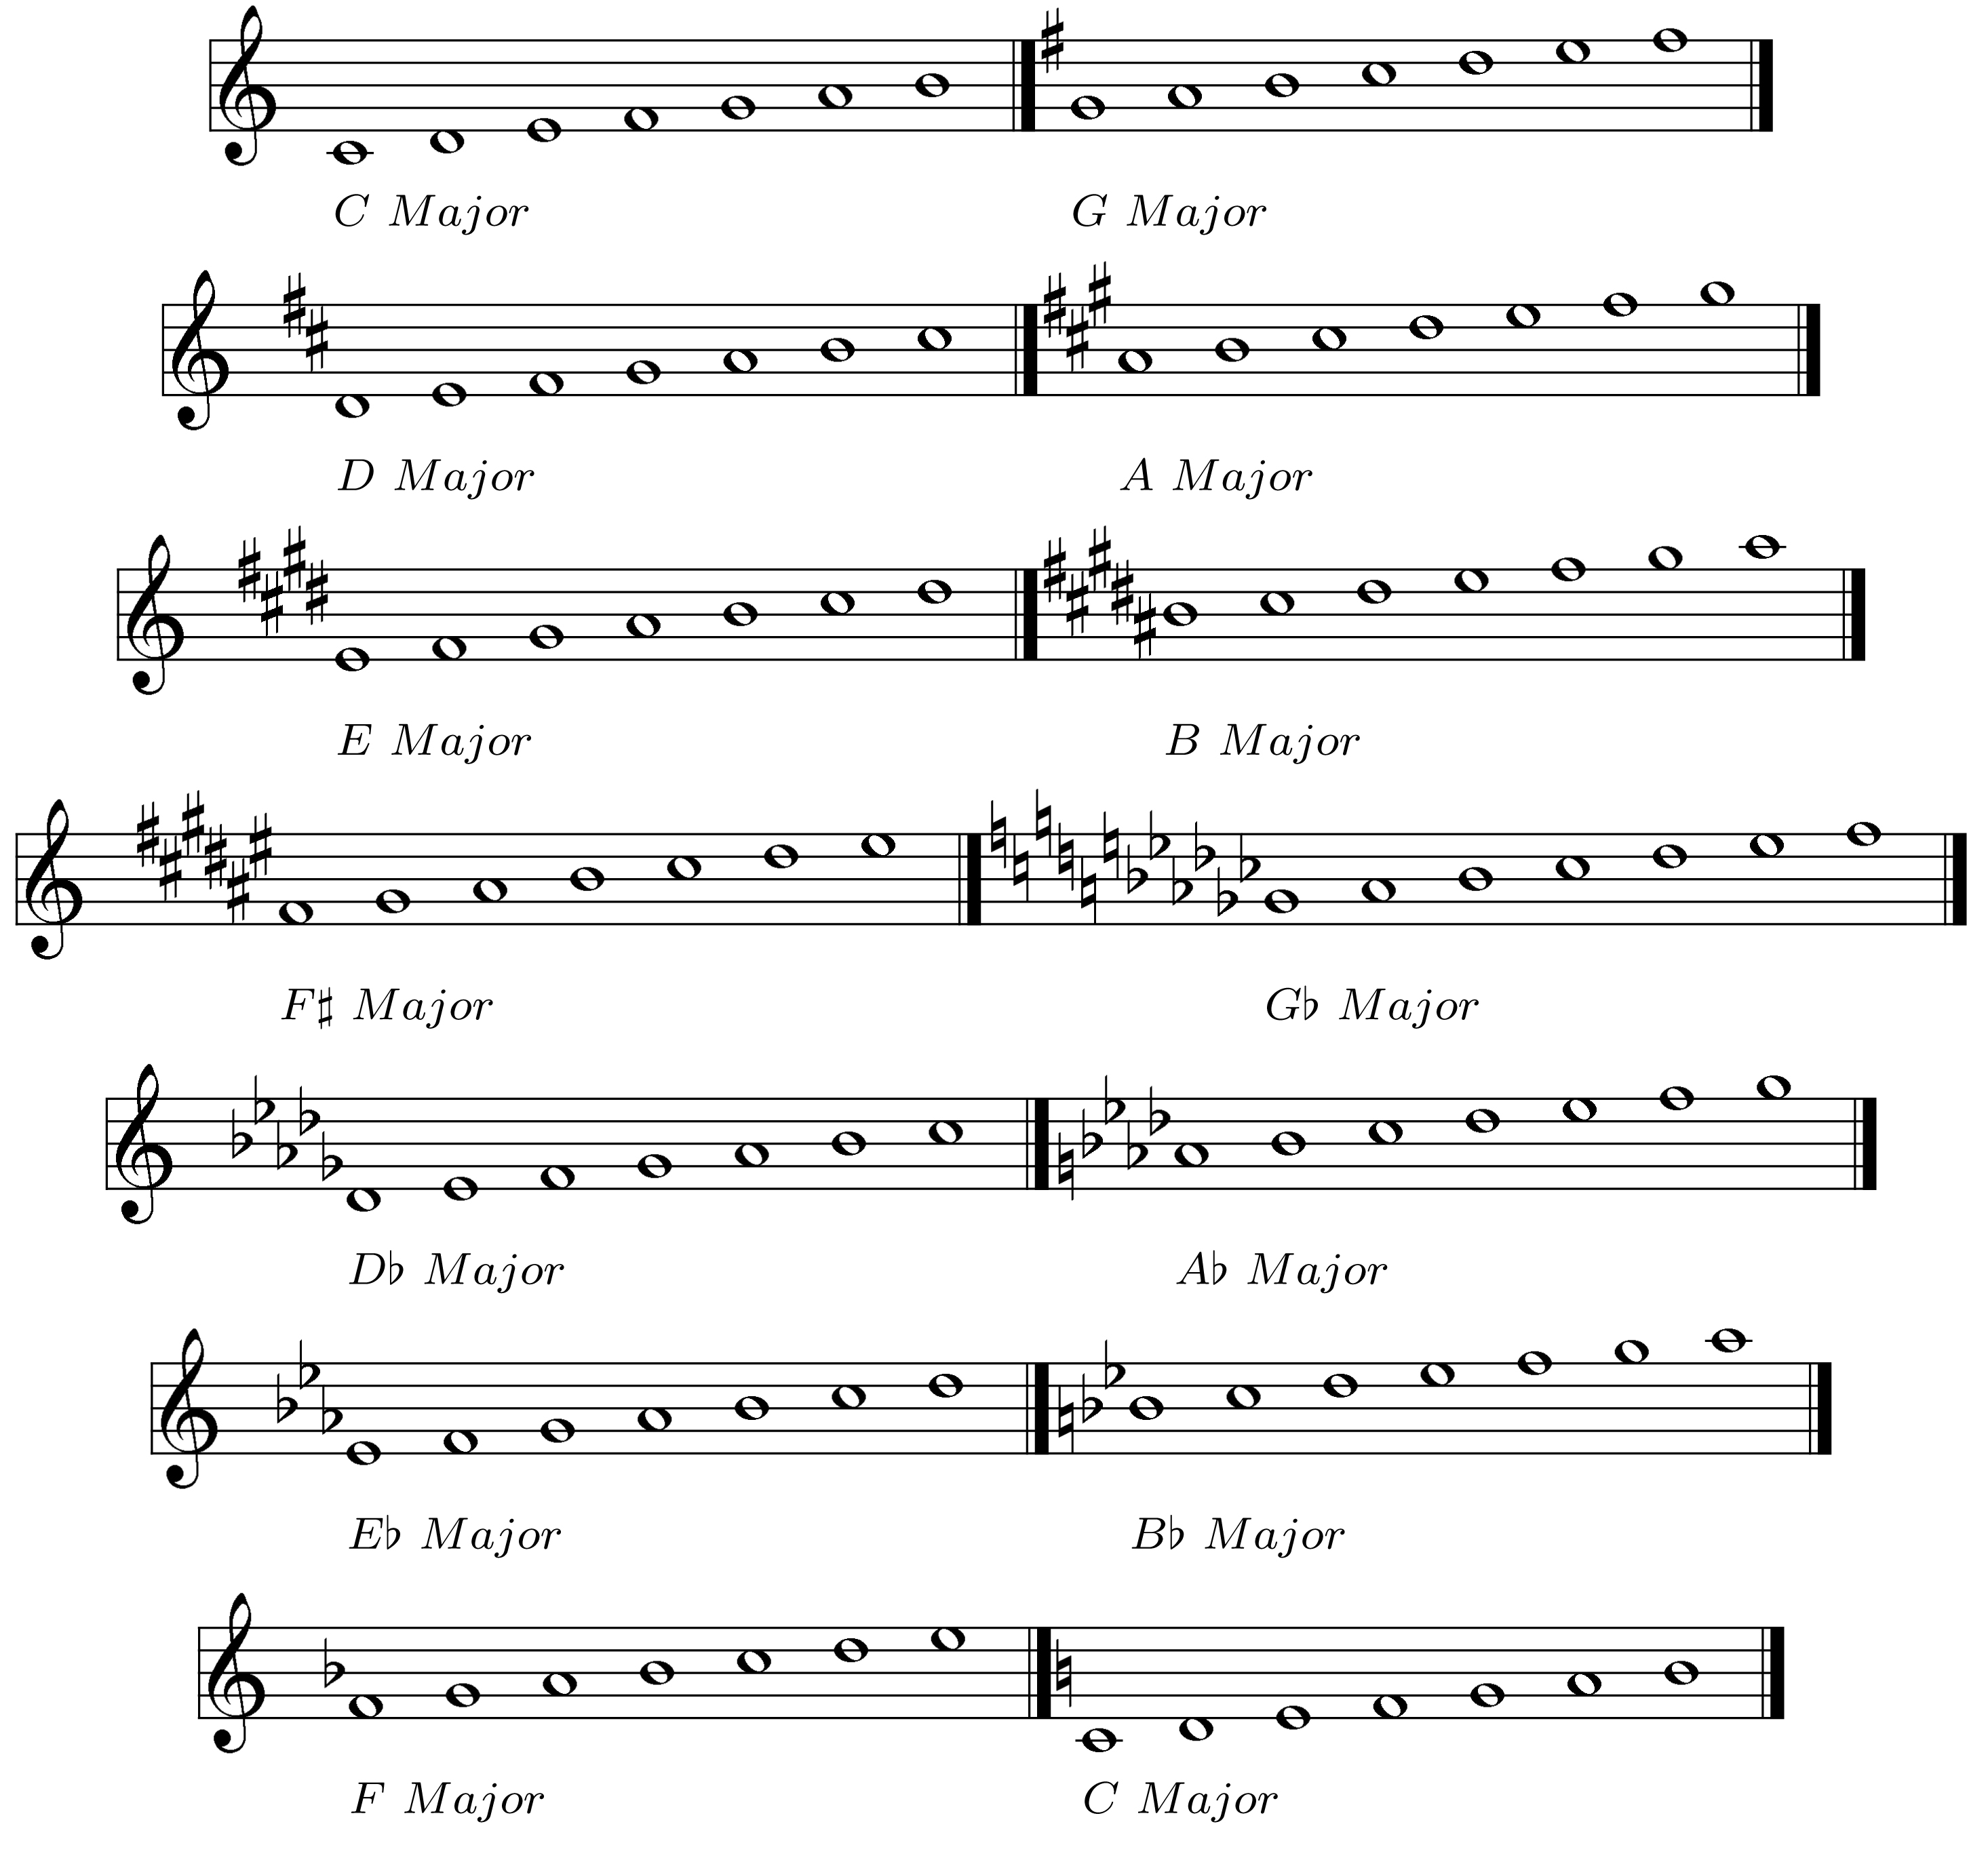
\includegraphics[scale=.6]{pitch_keys}
                \end{figure}
        \end{frame}
        
        \begin{frame}{pitch}{musical pitch --- key: circle of fifths}
            \scalebox{.9}
            {
                %\begin{figure}
                    \centering
                    
\begin{footnotesize}
\begin{picture}(80,85)
	\setcounter{iXOffset}{40} %radius
	\setcounter{iXBlockSize}{80}

	% circles
	\put(\value{iXOffset},\value{iXOffset}){\color[rgb]{0.8,0.8,0.8}\circle*{\value{iXBlockSize}}}
	\put(\value{iXOffset},\value{iXOffset}){\color[rgb]{0.5,0.5,0.5}\circle*{58}}
	\put(\value{iXOffset},\value{iXOffset}){\color[rgb]{0.8,0.8,0.8}\circle*{36}}
	
	\put(\value{iXOffset},\value{iXOffset}){\circle{\value{iXBlockSize}}}
	\put(\value{iXOffset},\value{iXOffset}){\circle{58}}
	\put(\value{iXOffset},\value{iXOffset}){\circle{36}}

	% radial lines	
	\put( 1.363, 29.6472){\line(0.9659, 0.2588){77.3}}
	\put( 1.363, 50.3528){\line(0.9659,-0.2588){77.3}}
	
	\put( 11.7157, 11.7157){\line(0.7071, 0.7071){56.5}}
	\put( 11.7157, 68.2843){\line(0.7071,-0.7071){56.5}}
	
	\put( 29.6472, 1.3630){\line(0.2588, 0.9659){20.7}}
	\put( 29.6472, 78.6370){\line(0.2588,-0.9659){20.7}}

	% major
	\put(37.5, 78){\text{\tiny{Major}}}
	
	\put(39, 73){\text{$C$}}

	\put(56, 68){\text{$G$}}
	\put(20, 68){\text{$F$}}

	\put(68, 55){\text{$D$}}
	\put(9, 55){\text{$B\flat$}}

	\put(73, 39){\text{$A$}}
	\put(4, 39){\text{$E\flat$}}

	\put(68, 23){\text{$E$}}
	\put(9, 22){\text{$A\flat$}}

	\put(56, 10){\text{$B$}}
	\put(20, 10){\text{$D\flat$}}

	\put(36, 5){\text{$G\flat\ / F\sharp$}}


	% minor
	\put(37.5, 67){\text{\tiny{minor}}}
	
	\put(39, 63){\text{$a$}}

	\put(51, 60){\text{$e$}}
	\put(28, 60){\text{$d$}}

	\put(60, 51){\text{$b$}}
	\put(19, 51){\text{$g$}}

	\put(62, 39){\text{$f\sharp$}}
	\put(16, 39){\text{$c$}}

	\put(60, 27.5){\text{$c\sharp$}}
	\put(19, 27){\text{$f$}}

	\put(51, 19){\text{$g\sharp$}}
	\put(27, 18){\text{$b\flat$}}

	\put(37, 15){\text{$e\flat\ / d\sharp$}}

	% accidentals

	\put(38.5, 56){\text{\tiny{accs.}}}

	\put(39, 51){\text{$0$}}

	\put(45, 50){\text{$1\sharp$}}
	\put(32.5, 49.5){\text{$1\flat$}}

	\put(50, 45){\text{$2\sharp$}}
	\put(28, 45){\text{$2\flat$}}

	\put(51, 39){\text{$3\sharp$}}
	\put(27, 39){\text{$3\flat$}}

	\put(49, 33){\text{$4\sharp$}}
	\put(28, 33){\text{$4\flat$}}

	\put(45, 29){\text{$5\sharp$}}
	\put(32.5, 29){\text{$5\flat$}}

	\put(39, 28){\text{$6\flat$}}
	\put(39, 25){\text{$6\sharp$}}
	
\end{picture}
\end{footnotesize}

                %\end{figure}
            }					
        \end{frame}
        
        \begin{frame}{pitch}{musical pitch --- chords}
            \begin{itemize}
                \item	simultaneous use of several pitches $\Rightarrow$ \textbf{chords}
                \item	usually constructed of (major/minor) thirds
                \begin{figure}[t]
                    \centering
                    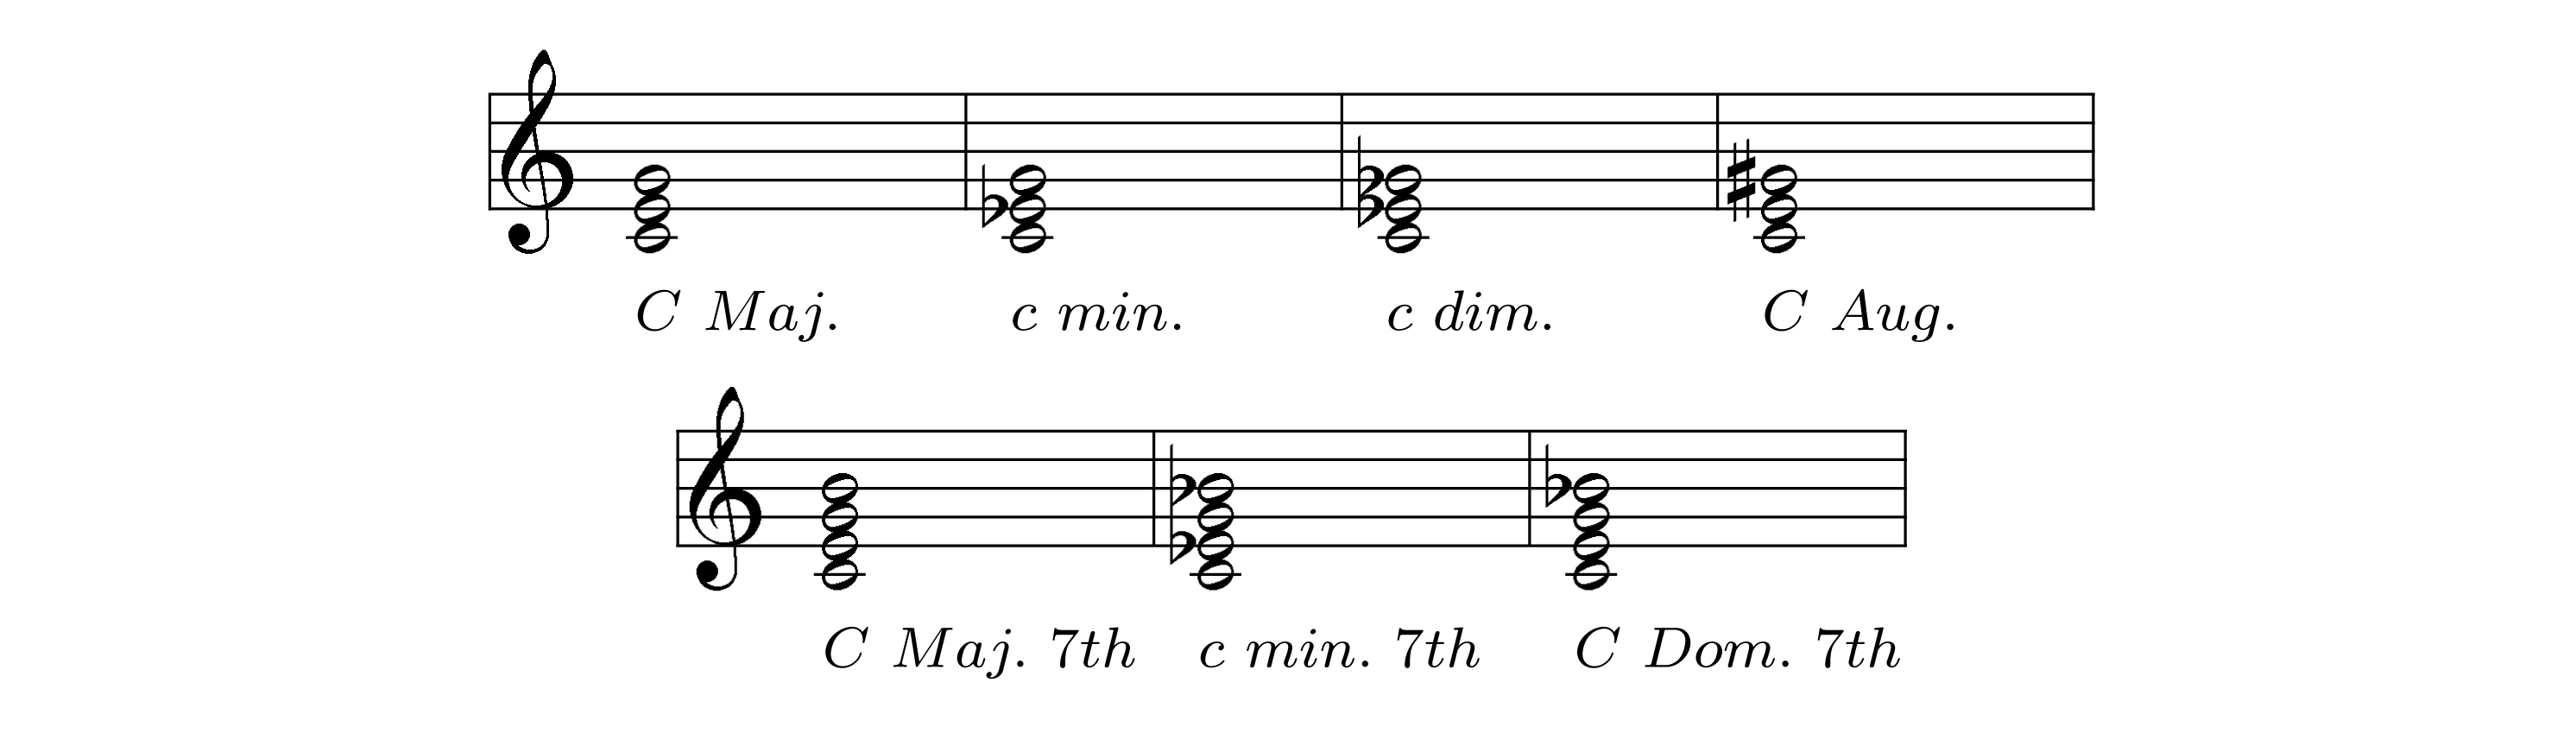
\includegraphics[scale=.7]{pitch_chords}
                \end{figure}
                \pause
                
                \item	note:
                        \begin{itemize}
                            \item	chord type independent of pitch doubling
                            \item	same label for keys and chords
                        \end{itemize}
            \end{itemize}
        \end{frame}
        
        \begin{frame}{pitch}{musical pitch --- chord inversion}
            \begin{itemize}
                \item	most common: root note is lowest note
                \item	otherwise: chord inversion
                \begin{figure}[t]
                    \centering
                    
\includegraphics{pitch_chordinversions}
                \end{figure}
                
            \end{itemize}
        \end{frame}
        
        \begin{frame}{pitch}{musical pitch --- harmony}
            \begin{itemize}
                \item	key and tonal context define chord's \textit{harmonic function}:
                \pause
                \begin{itemize}
                    \item	\textbf{tonic}:\\ chord on 1st scale degree (tonal center)
                    \item	\textbf{dominant}:\\ chord on 5th scale degree (often moves to tonic)
                    \item	\textbf{subdominant}:\\ chord on 4th scale degree
                    \item	\ldots
                \end{itemize}
            \end{itemize}
        \end{frame}
        
        \begin{frame}{pitch}{musical pitch --- MIDI pitch}
                \begin{eqnarray*}\label{eq:midi_pitch}
                    \mathfrak{p}(f) &=& 69 + 12\cdot\log_2\left(\frac{f}{f_{A4}}\right) \\
                    \pause
                    f(\mathfrak{p}) &=& f_{A4}\cdot2^{\frac{\mathfrak{p}-69}{12}}
                \end{eqnarray*}
                
                \pause
                MIDI pitch mapping to \textit{pitch class}
                \begin{equation*}\label{eq:pcidx}
                    \mathrm{PC}(\mathfrak{p}) = \mod(\mathfrak{p}, 12) 
                \end{equation*}
                
        \end{frame}
        
        \begin{frame}{pitch}{musical pitch --- (MIDI) pitch distance}
                \textbf{cent}: pitch distance between to frequencies
                \begin{footnotesize}
                \begin{eqnarray*}\label{eq:cent}
                    \Delta C(f_1,f_2)	&=& 100\cdot\big(\mathfrak{p}(f_1) - \mathfrak{p}(f_2)\big)\\
                                        \pause
                                        &=& 100\cdot\left(\left(69 + 12\cdot\log_2\left(\frac{f_1}{f_{A4}}\right)\right) - \left(69 + 12\cdot\log_2\left(\frac{f_2}{f_{A4}}\right)\right)\right)\\
                                        \pause
                                        &=& 1200\cdot\log_2\left( \frac{f_1}{f_2} \right) 
                \end{eqnarray*}
                \end{footnotesize}
                $\Rightarrow$ semitone $=\unit[100]{cents}$
        \end{frame}
        
        
        \begin{frame}{pitch}{musical pitch --- temperament}
            \begin{itemize}
                \item	equally tempered scale
                    \begin{equation*}
                        \frac{f_1}{f_2} = 2^{\nicefrac{N}{12}} 
                    \end{equation*}
                    \begin{itemize}
                        \item<2->	enharmonic equivalence: $C\sharp = D\flat$
                    \end{itemize}

                \item<3->	deviations of other scales
                    \begin{tiny}\begin{table}
                        \centering
                        \begin{tabular}{lcccccc} %{c|p{12mm}p{12mm}p{12mm}p{12mm}p{12mm}p{12mm}p{12mm}}
                            \\ \hline
                            \bf{\emph{Pitch Class}}	 & \bf{\emph{Equally}}	 & \bf{\emph{Pythagorean}}	 & \bf{\emph{Meantone}}	 & \bf{\emph{Diatonic Major}}	 & \bf{\emph{Diatonic Minor}}\\ 
                             \hline
                            \bf{$C$}	 & $0$	 & $0$	 & $0$	 & $0$	 & $0$\\
                            \bf{$C^\#$}	 & $0$	 & $-$	 & $-$	 & $-$	 & $-$\\
                            \bf{$D$}	 & $0$	 & $+3.9$	 & $-6.9$	 & $+3.9$	 & $+3.9$\\
                            \bf{$E^b$}	 & $0$	 & $-$	 & $-$	 & $-$	 & $+15.6$\\
                            \bf{$E$}	 & $0$	 & $+7.8$	 & $-13.7$	 & $-13.7$	 & $-$\\
                            \bf{$F$}	 & $0$	 & $-2.0$	 & $+3.4$	 & $-2.0$	 & $-2.0$\\
                            \bf{$F^\#$}	 & $0$	 & $-$	 & $-$	 & $-$	 & $-$\\
                            \bf{$G$}	 & $0$	 & $+2.0$	 & $-3.5$	 & $+2.0$	 & $+2.0$\\
                            \bf{$A^b$}	 & $0$	 & $-$	 & $-$	 & $-$	 & $+13.7$\\
                            \bf{$A$}	 & $0$	 & $+5.9$	 & $-10.2$	 & $-15.6$	 & $-$\\
                            \bf{$B^b$}	 & $0$	 & $-$	 & $-$ 	 & $-$	 & $+17.6$\\
                            \bf{$B$}	 & $0$	 & $+9.8$	 & $-17.1$	 & $-11.7$	 & $-$\\
                        \end{tabular}
                    \end{table}\end{tiny}			
            \end{itemize}
        \end{frame}
        
        \begin{frame}{pitch}{musical pitch --- intonation \& vibrato}
            \begin{itemize}
                \item	\textbf{expressive intonation}: deviation of pitch frequency from temperament depending on musical context
                        \begin{itemize}
                            \item	leading tones
                            \item	``pure'' intervals
                        \end{itemize}

                \item<2->	\textbf{vibrato}
                        \begin{itemize}
                            \item	periodic modulation around mean pitch
                            \pause
                            \item 	frequency: app. 4--10 \unit{Hz}, range: app. 20--300 \unit{cents}	
                        \end{itemize}
                \bigskip
                \item<3-> applies only to instruments with
                    \begin{itemize}
                        \item<4->   continuous frequency scales: vocals, string instruments, trombone, \ldots
                        \item<5->   other possibilities to adjust frequency: guitar, wind instruments, \ldots
                    \end{itemize}
            \end{itemize}
        \end{frame}
            
   \section[summary]{lecture summary}
        \begin{frame}{summary}{lecture content}
            \begin{enumerate}
                \item   how can concepts of pitch perception and knowledge of musical conventions be important in audio content analysis? name examples.
                \smallskip
                \item<2->   you hear a sound with one pitch? what relation do the frequencies it contains usually have?
                \smallskip
                \item<3->   what are the two dimensions of human pitch perception?
                \smallskip
                \item<4->   describe key relationships according to the circle-of-fifths model
                \smallskip
                \item<5->   what is the ``unit'' cent and how does it relate to the MIDI pitch 
            \end{enumerate}
        \end{frame}
\end{document}

